\documentclass{paper}
\usepackage{amsmath}
\usepackage{blindtext}
\usepackage[utf8]{inputenc}
\usepackage{amssymb}
\usepackage{setspace}
\usepackage{graphicx}
\usepackage{geometry}
\usepackage{listings}
\usepackage{float}
\usepackage{natbib}
\usepackage{multicol}

\geometry{left = 1in, right =1in,top=1in, bottom = 1in}
\begin{document}
\newcommand*{\be}{\mathbb{E}}
\newcommand*{\bv}{\mathbb{V}}
\lstset{showspaces = false, showstringspaces = false}
\linespread{2}
\title{Numerical Comparative Dynamics: Ball Python Breeding}
\author{Donald DiJacklin}
\maketitle
\bibliographystyle{chicago}
\begin{spacing}{1.5}
\section*{Background}
	\indent\indent Breeding animals in general is an extremely time dependent system since the animals you have now were generated by animals you had previously and a slightly different occurence in a previous time period can drastically change the future time periods. For example, having 5 new-borns in one period versus having 4, something that could easily happen by chance, supposing that each new-born will have 3 offspring per time period results in 4 more animals than there would have been in the next time period. In two time periods there will be 16 more animals than there would have been. This is a massive simplification of any actual breeding system in many ways, one of which is that breeder's aren't just trying to get more animals in most cases, they're also trying to get better animals from breeding.\\
	As one that has some domain knowledge in Ball Python (\textit{python regius}) breeding, I am going to study how slight differences in a Ball Python breeding system affect profits, using simulation. There are several facets of Ball Python breeding that will factor heavily in this project, the most important of which is that Ball Python prices are largely determined by their `morphs', i.e. the traits they possess, such as the snake on the left expresses no morphs, and sells for about \$20, and the snake on the right expresses the trait called Pastel, and sells for about \$40 for a male.\\
	\begin{multicols}{2}
	\begin{figure}[H]
	\centering
	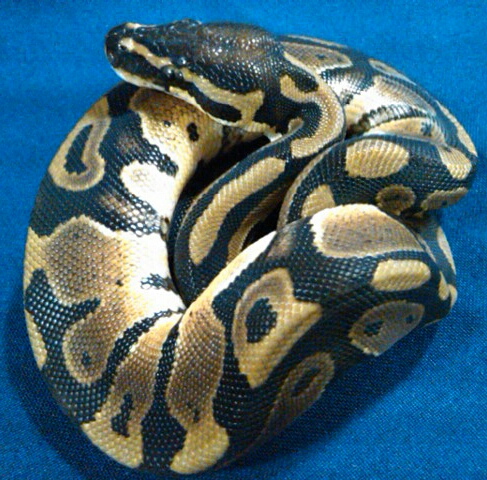
\includegraphics[width=.5\textwidth, height = 62mm]{Normal.jpg}
	\end{figure}
	\begin{figure}[H]
	\centering
	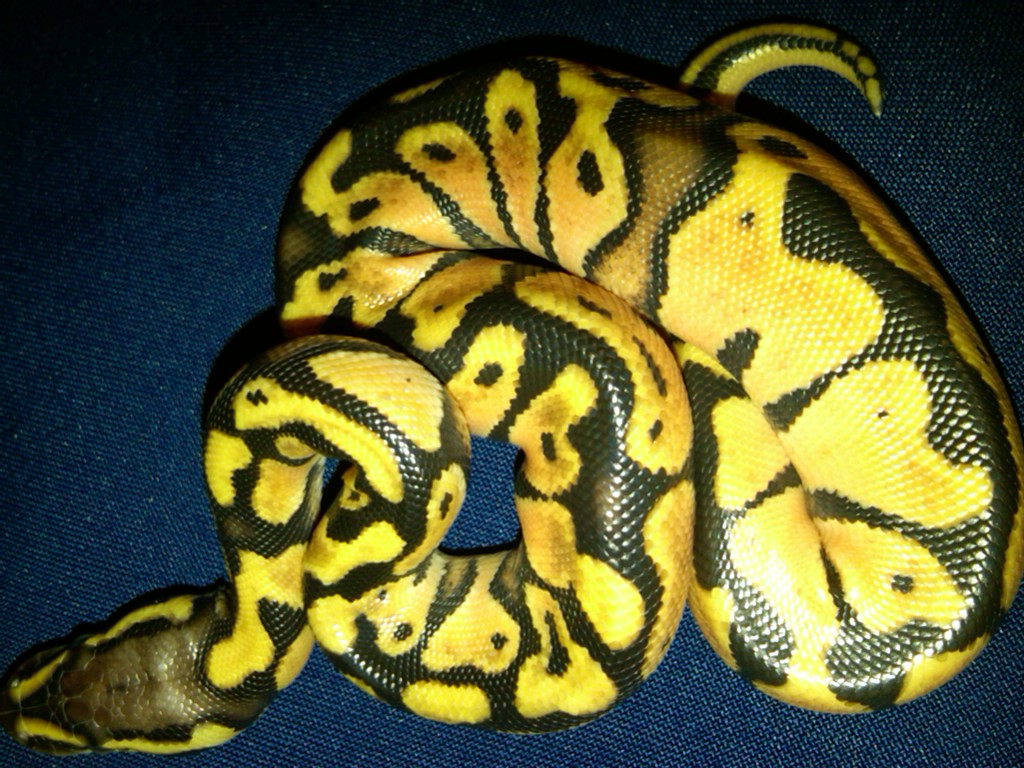
\includegraphics[width=.5\textwidth]{Pastel.jpg}
	\end{figure}
	\end{multicols}
	
	
	Other important aspects that will be used in this project are:
	\begin{itemize}
	\item It costs a breeder about \$80 per year to maintain a Ball Python.
	\item A male Ball Python can inseminate up to five females per year.
	\item A female Ball Python can be inseminated up to once per year.
	\item A male will take about one year to reach sexual maturity.
	\item A female will take about two years to reach sexual maturity.
	\item About 60\% of pairings will result in a set of eggs, called a clutch.
	\end{itemize}

	\end{spacing}
	\bibliography{References}
	\nocite{*}
\begin{spacing}{1.5}
\section*{Models}
	\indent\indent One may wonder why I'm not using a dynamic program to answer my questions, which is certainly a reasonable question. The answer is that I started that way, and was at a point where I had three separate indices and was considering a fourth, while I was nowhere close to actually modeling the system even discounting inbreeding. So I turned to the following: in each time period a snake breeder needs to make two decisions, firstly, which males to breed with which females. Secondly, which snakes to keep and which to sell off down to their carrying capacity. I'm going to answer these questions in a simulation in order to come up with average profit per period given the parameters of the system.\\
	\indent As for the first decision, a higher value male paired with a higher value female generates higher value babies, with the caveat that inbreeding is restricted. According to \cite{becker}, aside from the inbreeding, the optimal matching should be PAM (positive assortative matching).\\
	\indent As for the second decision, shown below is the integer program to solve for the best snakes to keep given a capacity of 15. Where R is the matrix where the ijth entry is the expected revenue from breeding male i and female j. X is the choice matrix where a 1 as the ijth entry means that you should breed male i and female j in the next period. y is a vector that shows which males to keep, and z is a vector that shows which females to keep.
	\begin{align*}
      \max_{\mathbf{X},\mathbf{y},\mathbf{z}}\{ &\sum_{i\in I}\mathbf R_i (\mathbf X_i)^T - 80\mathbf y^T\mathbf 1_I - 80\mathbf z^T\mathbf 1_J \}\\
      s.t. \quad& \mathbf X\mathbf 1_J \leq 5\mathbf 1_I \\
      & \mathbf X^T \mathbf 1_I \leq \mathbf1_J\\
      & \mathbf X \mathbf1_J\leq M\mathbf y\\
      & \mathbf X^T\mathbf 1_I \leq M\mathbf z\\
      & \mathbf y^T\mathbf 1_I + \mathbf z^T\mathbf 1_J \leq 15\\
      & X_{ij}, y_i, z_j \in \{0,1\}
    \end{align*}
   \section*{Data}
   	There are three main sources for the data in this paper.\\First, I have obtained all the bullet-pointed information in the first section from my brother, a small to medium-sized snake breeder. \\Second, I have obtained data on snake prices from snake breeders at the Tampa Florida Repticon by going to many breeders and asking to take pictures of their display. Data from that source was transcribed in the form:\\
   	Sex, List of traits, Price\\
   	and has been manipulated into all binary variables, 1 if the snake has a trait, 0 if it doesn't, except price. Any traits with 2 or less observations and snakes that have them will be trimmed from the data set. These binary variables will then be used to train a regression model to identify the price of the individual traits.\\
   	The third source that I'm working on getting is from the snake breeding company known as The Snake Keeper, which will be about clutch sizes, so that I can incorporate the distribution of clutch sizes into my model. This data will not be strictly neccessary to make my program work, but it will make the results closer to possible real life scenarios.

\end{spacing}

\end{document}